% Options for packages loaded elsewhere
\PassOptionsToPackage{unicode}{hyperref}
\PassOptionsToPackage{hyphens}{url}
%
\documentclass[
  man]{apa6}
\usepackage{amsmath,amssymb}
\usepackage{lmodern}
\usepackage{iftex}
\ifPDFTeX
  \usepackage[T1]{fontenc}
  \usepackage[utf8]{inputenc}
  \usepackage{textcomp} % provide euro and other symbols
\else % if luatex or xetex
  \usepackage{unicode-math}
  \defaultfontfeatures{Scale=MatchLowercase}
  \defaultfontfeatures[\rmfamily]{Ligatures=TeX,Scale=1}
\fi
% Use upquote if available, for straight quotes in verbatim environments
\IfFileExists{upquote.sty}{\usepackage{upquote}}{}
\IfFileExists{microtype.sty}{% use microtype if available
  \usepackage[]{microtype}
  \UseMicrotypeSet[protrusion]{basicmath} % disable protrusion for tt fonts
}{}
\makeatletter
\@ifundefined{KOMAClassName}{% if non-KOMA class
  \IfFileExists{parskip.sty}{%
    \usepackage{parskip}
  }{% else
    \setlength{\parindent}{0pt}
    \setlength{\parskip}{6pt plus 2pt minus 1pt}}
}{% if KOMA class
  \KOMAoptions{parskip=half}}
\makeatother
\usepackage{xcolor}
\IfFileExists{xurl.sty}{\usepackage{xurl}}{} % add URL line breaks if available
\IfFileExists{bookmark.sty}{\usepackage{bookmark}}{\usepackage{hyperref}}
\hypersetup{
  pdftitle={Supplementary Figures DateLife: leveraging databases and analytical tools to reveal the dated Tree of Life},
  pdfauthor={Luna L. Sánchez Reyes1,2, Emily Jane McTavish1, \& Brian O'Meara2},
  pdflang={en-EN},
  hidelinks,
  pdfcreator={LaTeX via pandoc}}
\urlstyle{same} % disable monospaced font for URLs
\usepackage{graphicx}
\makeatletter
\def\maxwidth{\ifdim\Gin@nat@width>\linewidth\linewidth\else\Gin@nat@width\fi}
\def\maxheight{\ifdim\Gin@nat@height>\textheight\textheight\else\Gin@nat@height\fi}
\makeatother
% Scale images if necessary, so that they will not overflow the page
% margins by default, and it is still possible to overwrite the defaults
% using explicit options in \includegraphics[width, height, ...]{}
\setkeys{Gin}{width=\maxwidth,height=\maxheight,keepaspectratio}
% Set default figure placement to htbp
\makeatletter
\def\fps@figure{htbp}
\makeatother
\setlength{\emergencystretch}{3em} % prevent overfull lines
\providecommand{\tightlist}{%
  \setlength{\itemsep}{0pt}\setlength{\parskip}{0pt}}
\setcounter{secnumdepth}{-\maxdimen} % remove section numbering
% Make \paragraph and \subparagraph free-standing
\ifx\paragraph\undefined\else
  \let\oldparagraph\paragraph
  \renewcommand{\paragraph}[1]{\oldparagraph{#1}\mbox{}}
\fi
\ifx\subparagraph\undefined\else
  \let\oldsubparagraph\subparagraph
  \renewcommand{\subparagraph}[1]{\oldsubparagraph{#1}\mbox{}}
\fi
\ifLuaTeX
\usepackage[bidi=basic]{babel}
\else
\usepackage[bidi=default]{babel}
\fi
\babelprovide[main,import]{english}
% get rid of language-specific shorthands (see #6817):
\let\LanguageShortHands\languageshorthands
\def\languageshorthands#1{}
\DeclareUnicodeCharacter{0301}{*************************************}

% leave the figure captions outside\ caption{} if you want them
% to be formatted in the same way as the general text (double spaced and linenumbered)
% line numbers for captions trick from https://latex.org/forum/viewtopic.php?t=34614

\usepackage{ragged2e}

\usepackage{caption}

\usepackage{lineno}
\DeclareCaptionFont{linenumbers}{\internallinenumbers}

\usepackage{float}
\restylefloat{table}

\captionsetup[figure]{font+=linenumbers, labelfont={sc}, labelformat={default}, labelsep=period, name={Supplementary Figure}}

\captionsetup[table]{font+=linenumbers, labelfont={sc}, labelformat={default}, labelsep=period, name={Supplementary Table}}

% Manuscript styling
\usepackage{upgreek}
\captionsetup{font=singlespacing,justification=justified}

% Table formatting
\usepackage{longtable}
\usepackage{lscape}
% \usepackage[counterclockwise]{rotating}   % Landscape page setup for large tables
\usepackage{multirow}		% Table styling
\usepackage{tabularx}		% Control Column width
\usepackage[flushleft]{threeparttable}	% Allows for three part tables with a specified notes section
\usepackage{threeparttablex}            % Lets threeparttable work with longtable

% Create new environments so endfloat can handle them
% \newenvironment{ltable}
%   {\begin{landscape}\centering\begin{threeparttable}}
%   {\end{threeparttable}\end{landscape}}
\newenvironment{lltable}{\begin{landscape}\centering\begin{ThreePartTable}}{\end{ThreePartTable}\end{landscape}}

% Enables adjusting longtable caption width to table width
% Solution found at http://golatex.de/longtable-mit-caption-so-breit-wie-die-tabelle-t15767.html
\makeatletter
\newcommand\LastLTentrywidth{1em}
\newlength\longtablewidth
\setlength{\longtablewidth}{1in}
\newcommand{\getlongtablewidth}{\begingroup \ifcsname LT@\roman{LT@tables}\endcsname \global\longtablewidth=0pt \renewcommand{\LT@entry}[2]{\global\advance\longtablewidth by ##2\relax\gdef\LastLTentrywidth{##2}}\@nameuse{LT@\roman{LT@tables}} \fi \endgroup}

% \setlength{\parindent}{0.5in}
% \setlength{\parskip}{0pt plus 0pt minus 0pt}

% Overwrite redefinition of paragraph and subparagraph by the default LaTeX template
% See https://github.com/crsh/papaja/issues/292
\makeatletter
\renewcommand{\paragraph}{\@startsection{paragraph}{4}{\parindent}%
  {0\baselineskip \@plus 0.2ex \@minus 0.2ex}%
  {-1em}%
  {\normalfont\normalsize\bfseries\itshape\typesectitle}}

\renewcommand{\subparagraph}[1]{\@startsection{subparagraph}{5}{1em}%
  {0\baselineskip \@plus 0.2ex \@minus 0.2ex}%
  {-\z@\relax}%
  {\normalfont\normalsize\itshape\hspace{\parindent}{#1}\textit{\addperi}}{\relax}}
\makeatother

% \usepackage{etoolbox}
\makeatletter
\patchcmd{\HyOrg@maketitle}
  {\section{\normalfont\normalsize\abstractname}}
  {\section*{\normalfont\normalsize\abstractname}}
  {}{\typeout{Failed to patch abstract.}}
\patchcmd{\HyOrg@maketitle}
  {\section{\protect\normalfont{\@title}}}
  {\section*{\protect\normalfont{\@title}}}
  {}{\typeout{Failed to patch title.}}
\makeatother

\usepackage{xpatch}
\makeatletter
\xapptocmd\appendix
  {\xapptocmd\section
    {\addcontentsline{toc}{section}{\appendixname\ifoneappendix\else~\theappendix\fi\\: #1}}
    {}{\InnerPatchFailed}%
  }
{}{\PatchFailed}
\DeclareDelayedFloatFlavor{ThreePartTable}{table}
\DeclareDelayedFloatFlavor{lltable}{table}
\DeclareDelayedFloatFlavor*{longtable}{table}
\makeatletter
\renewcommand{\efloat@iwrite}[1]{\immediate\expandafter\protected@write\csname efloat@post#1\endcsname{}}
\makeatother
\usepackage{csquotes}
\ifLuaTeX
  \usepackage{selnolig}  % disable illegal ligatures
\fi

\title{Supplementary Figures \linebreak DateLife: leveraging databases and analytical tools to reveal the dated Tree of Life}
\author{Luna L. Sánchez Reyes\textsuperscript{1,2}, Emily Jane McTavish\textsuperscript{1}, \& Brian O'Meara\textsuperscript{2}}
\date{}


\shorttitle{DateLife Supplementary Figures}

\authornote{

Correspondence concerning this article should be addressed to Luna L. Sánchez Reyes, . E-mail: \href{mailto:sanchez.reyes.luna@gmail.com}{\nolinkurl{sanchez.reyes.luna@gmail.com}}

}

\affiliation{\vspace{0.5cm}\textsuperscript{1} Science and Engineering Building 1, School of Natural Sciences, University of California, Merced\\\textsuperscript{2} Department of Ecology and Evolutionary Biology, University of Tennessee, Knoxville}

\begin{document}
\maketitle


%%%%%%%%%%%%%%%%%%%%%%%%%%%%%%%%%%%%%%%%%%%%%%%%%%%%%%%%%%%%%%%%%%
%%%%%%%%%%%%%%%%    FIGURE CROSS VALIDATION    %%%%%%%%%%%%%%%%%%%
%%%%%%%%%%%%%%%%%%%%%%%%%%%%%%%%%%%%%%%%%%%%%%%%%%%%%%%%%%%%%%%%%%

\begin{figure}[!h]
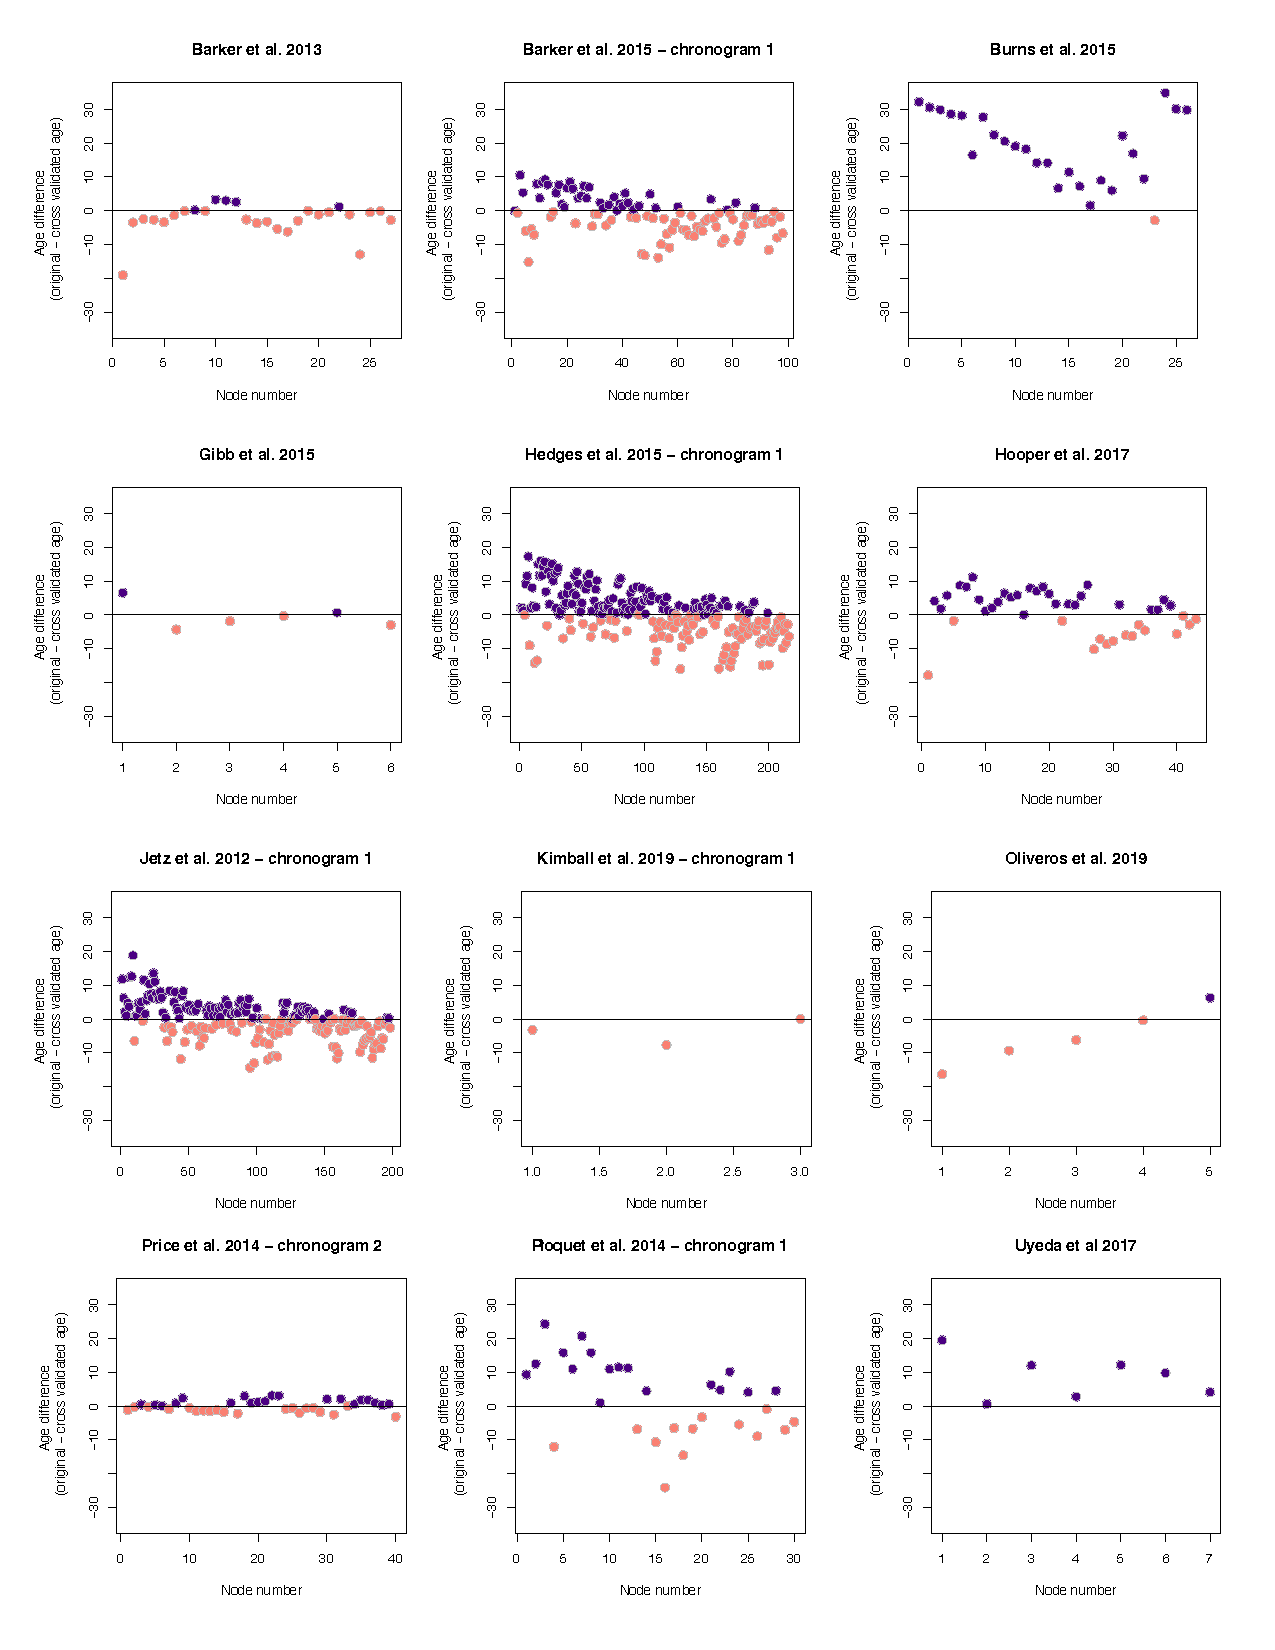
\includegraphics{../figures/figure-cross-validation/fig-cross-validation-xy-plots-diffs.pdf}
\caption{Results from cross validation analysis. Each plot shows the difference between the original age estimated and those obtained with a DateLife analysis, per node.}
\label{fig:cvXYdiffs}
\end{figure}

%%%%%%%%%%%%%%%%%%%%%%%%%%%%%%%%%%%%%%%%%%%%%%%%%%%%%%%%%%%%%%%%%%
%%%%%%%%%%%%%%%%   CROSS VALIDATION CHRONOGRAMS   %%%%%%%%%%%%%%%%
%%%%%%%%%%%%%%%%%%%%%%%%%%%%%%%%%%%%%%%%%%%%%%%%%%%%%%%%%%%%%%%%%%

\begin{figure}[!h]
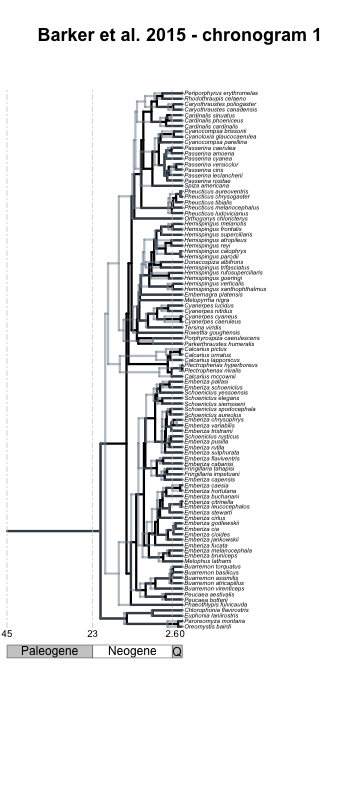
\includegraphics{../figures/figure-cross-validation/cross_validation_2.png}
\caption{Cross validation of Barker et al. (\protect\hyperlink{ref-barker2015new}{2015}) chronogram 1. The chronogram shown in black corresponds to the dates published in the original study. The gray chronogram corresponds to the same tree topology dated with BLADJ using node ages from all other source chronograms as secondary calibrations.}
\label{fig:cv2}
\end{figure}

\begin{figure}[!h]
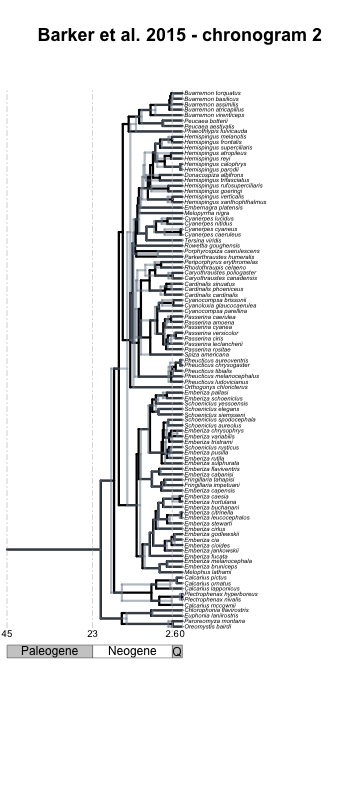
\includegraphics{../figures/figure-cross-validation/cross_validation_3.png}
\caption{Cross validation of Barker et al. (\protect\hyperlink{ref-barker2015new}{2015}) chronogram 1. The chronogram shown in black corresponds to the dates published in the original study. The gray chronogram corresponds to the same tree topology dated with BLADJ using node ages from all other source chronograms as secondary calibrations.}
\label{fig:cv3}
\end{figure}

\begin{figure}[!h]
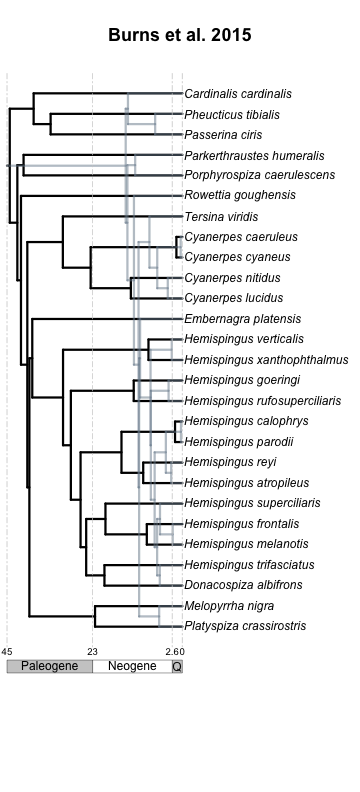
\includegraphics{../figures/figure-cross-validation/cross_validation_4.png}
\caption{Cross validation of Burns et al. (\protect\hyperlink{ref-burns2014phylogenetics}{2014}) chronogram. The chronogram shown in black corresponds to the dates published in the original study. The gray chronogram corresponds to the same tree topology dated with BLADJ using node ages from all other source chronograms as secondary calibrations.}
\label{fig:cv4}
\end{figure}

\begin{figure}[!h]
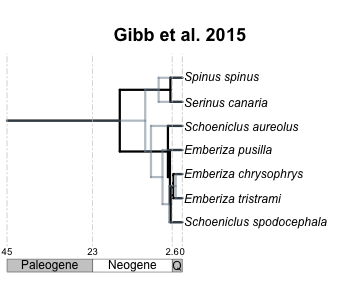
\includegraphics{../figures/figure-cross-validation/cross_validation_6.png}
\caption{Cross validation of Gibb et al. (\protect\hyperlink{ref-gibb2015new}{2015}), chronogram. The chronogram shown in black corresponds to the dates published in the original study. The gray chronogram corresponds to the same tree topology dated with BLADJ using node ages from all other source chronograms as secondary calibrations.}
\label{fig:cv6}
\end{figure}

\begin{figure}[!h]
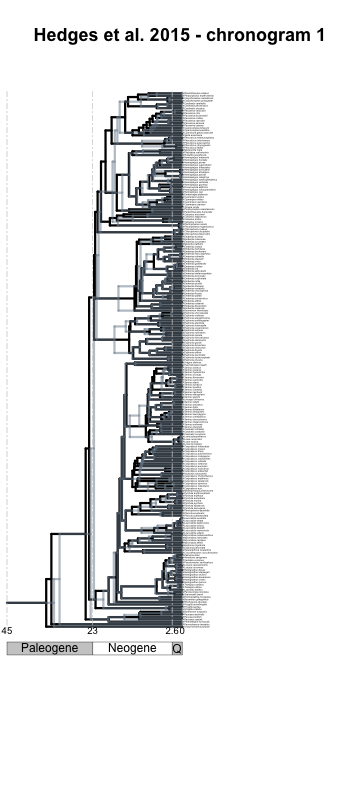
\includegraphics{../figures/figure-cross-validation/cross_validation_7.png}
\caption{Cross validation of Hedges et al. (\protect\hyperlink{ref-Hedges2015}{2015}) chronogram 1. The chronogram shown in black corresponds to the dates published in the original study. The gray chronogram corresponds to the same tree topology dated with BLADJ using node ages from all other source chronograms as secondary calibrations.}
\label{fig:cv7}
\end{figure}

\begin{figure}[!h]
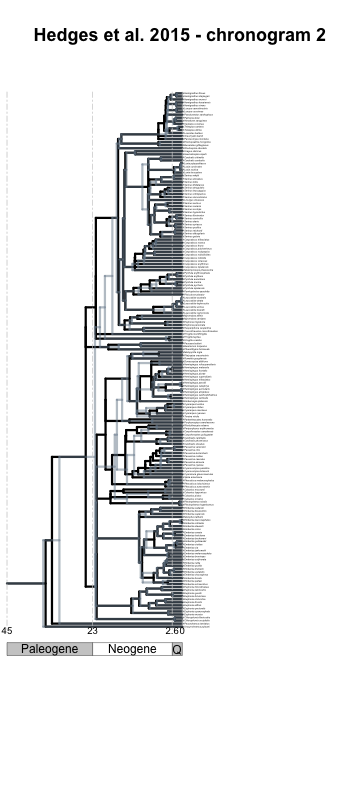
\includegraphics{../figures/figure-cross-validation/cross_validation_8.png}
\caption{Cross validation of Hedges et al. (\protect\hyperlink{ref-Hedges2015}{2015}) chronogram 2. The chronogram shown in black corresponds to the dates published in the original study. The gray chronogram corresponds to the same tree topology dated with BLADJ using node ages from all other source chronograms as secondary calibrations.}
\label{fig:cv8}
\end{figure}

\begin{figure}[!h]
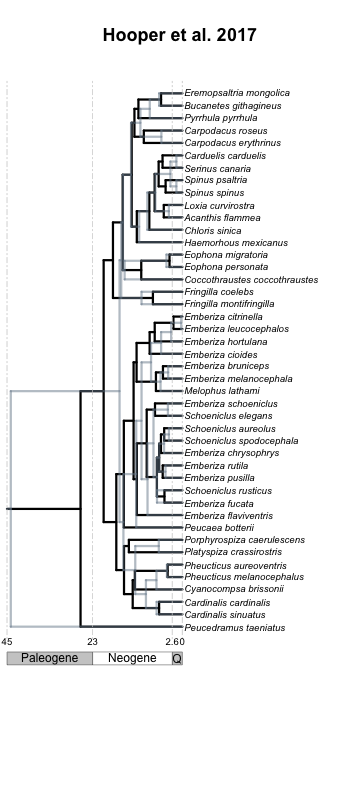
\includegraphics{../figures/figure-cross-validation/cross_validation_9.png}
\caption{Cross validation of Hooper and Price (\protect\hyperlink{ref-hooper2017chromosomal}{2017}) chronogram. The chronogram shown in black corresponds to the dates published in the original study. The gray chronogram corresponds to the same tree topology dated with BLADJ using node ages from all other source chronograms as secondary calibrations.}
\label{fig:cv9}
\end{figure}

\begin{figure}[!h]
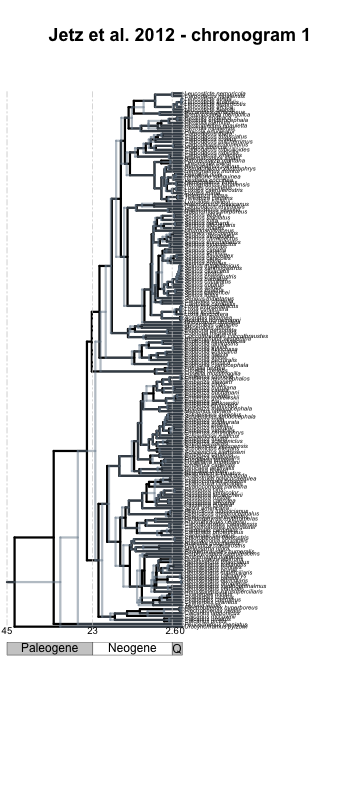
\includegraphics{../figures/figure-cross-validation/cross_validation_10.png}
\caption{Cross validation of Jetz et al. (\protect\hyperlink{ref-Jetz2012}{2012}) chronogram 1. The chronogram shown in black corresponds to the dates published in the original study. The gray chronogram corresponds to the same tree topology dated with BLADJ using node ages from all other source chronograms as secondary calibrations.}
\label{fig:cv10}
\end{figure}

\end{document}
